%%%%%%%%%%%%%%%%%%%%%%%%%%%%%%%%%%%%%%%%%%%%%%%%%%%%%%%%%%%%%%%%%%%%%%%%%
% All the content is in one file because I do not expect multiple editors.
%%%%%%%%%%%%%%%%%%%%%%%%%%%%%%%%%%%%%%%%%%%%%%%%%%%%%%%%%%%%%%%%%%%%%%%%%

\documentclass[11pt]{article}

%%%%%%%%%%%%%%%%%%%%%%%%%%%%%%%%%%%%%%%%%%%%%%%%%%%%%%%%%%%%%%%%%%%%%%%%%
%% packages

\usepackage{latexsym}
\usepackage{algorithm}
\usepackage{algorithmic}
\usepackage{graphicx}
\usepackage{subfigure}
\usepackage[T1]{fontenc}
% \usepackage{mathptmx}
% \usepackage{newcent}
\usepackage{fouriernc}
%\usepackage{times}
\usepackage{amsmath}
\usepackage{amssymb}
\usepackage{amsfonts}
\usepackage{fullpage}
% \usepackage{complexity}
\usepackage{hyphenat}
\usepackage{multirow}

\usepackage{enumitem}
% \usepackage[lite, subscriptcorrection]{mtpro2}

\usepackage[mathscr]{euscript}

\renewcommand{\P}{\mathbb{P}}
\newcommand{\E}{\mathbb{E}}
\newcommand{\Q}{\mathbb{Q}}
\newcommand{\R}{\mathbb{R}}
\newcommand{\Z}{\mathbb{Z}}
\newcommand{\N}{\mathbb{N}}
\newcommand{\C}{\mathbb{C}}
\newcommand{\K}{\mathbb{K}}
\newcommand{\cA}{\mathscr A}
\newcommand{\cF}{\mathcal F}
\newcommand{\cB}{\mathscr B}
\newcommand{\cM}{\mathscr M}
\newcommand{\cG}{\mathscr G}
\newcommand{\cP}{\mathscr P}
\newcommand{\cL}{\mathscr L}
\newcommand{\cX}{\mathscr X}
\newcommand{\cZ}{\mathscr Z}
\newcommand{\cE}{\mathscr E}
\newcommand{\cN}{\mathscr N}
\newcommand{\cT}{\mathscr T}
\newcommand{\ran}{\text{ran}}
\newcommand{\dom}{\text{dom}}
\newcommand{\supp}{\text{supp}}
\newcommand{\eps}{\varepsilon}
\newcommand{\var}{\text{Var}}
\newcommand{\ind}{{\mathbf 1}}

%%%%%%%%%%%%%%%%%%%%%%%%%%%%%%%%%%%%%%%%%%%%%%%%%%%%%%%%%%%%%%%%%%%%%%%%%
%% basic definitions, environments

\newtheorem{theorem}{Theorem}
\newtheorem{lemma}{Lemma}
\newtheorem{corollary}[theorem]{Corollary}
\newtheorem{definition}{Definition}
\newtheorem{property}{Property}
\newtheorem{observation}{Observation}
\newtheorem{remark}{Remark}

\newenvironment{proof}
        {\noindent {\em Proof.}~~~} %\\
        {\begin{flushright}$\Box$\end{flushright}}

\addtolength{\oddsidemargin}{-0.25in}
\addtolength{\evensidemargin}{-0.25in}
\addtolength{\textwidth}{0.5in}
\addtolength{\topmargin}{-.25in}
\addtolength{\textheight}{0.75in}	

%%%%%%%%%%%%%%%%%%%%%%%%%%%%%%%%%%%%%%%%%%%%%%%%%%%%%%%%%%%%%%%%%%%%%%%%%
%% title details

\title{
  Written Assignment \#2 \\[0.5em]
  \large
  Vancouver Summer Program 2019 -- Algorithms -- UBC \\
  \vspace*{0.2in} \hrule
}

%\author{
%	Sathish Gopalakrishnan
%}

\date{}

%%%%%%%%%%%%%%%%%%%%%%%%%%%%%%%%%%%%%%%%%%%%%%%%%%%%%%%%%%%%%%%%%%%%%%%%%

\begin{document}

\maketitle

\setlength{\baselineskip}{0.90\baselineskip}

%%%%%%%%%%%%%%%%%%%%%%%%%%%%%%%%%%%%%%%%%%%%%%%%%%%%%%%%%%%%%%%%%%%%%%%%%
%% the abstract

%% no abstract needed

%%%%%%%%%%%%%%%%%%%%%%%%%%%%%%%%%%%%%%%%%%%%%%%%%%%%%%%%%%%%%%%%%%%%%%%%%

\pagestyle{empty}

\vspace*{-0.75in}

% \straightbraces

\begin{itemize}
\item You should work with a partner.
\item You must typeset your solutions.
\item Submit your work using Gradescope by {\bf 5:00 p.m. on July 26}.
\item \textbf{Notation.} $\N = \{1,2,\dotsc\} \subset \{0,1,2,\dotsc\} = \Z_{+}$, and $\R_{+} = [0,\infty)$.
\end{itemize}

\hrule

\begin{enumerate}
\item {\bf Path Finding in an Hourglass Map.} In an hourglass map (example below) a path is marked. A path always starts at the first row and ends at the last row. Each cell in the path (except the first) should be directly below to the left or right of the cell in the path in the previous row. The value of a path is the sum of the values in each cell in the path.

A path is described with an integer representing the starting point in the first row (the leftmost cell being 1) followed by a direction string containing the letters L and R, telling whether to go to the left or right. For instance, the path below is described as 3 RRRLLRRRLR.

	\begin{figure}[h] \centering
		\scalebox{0.4}{
			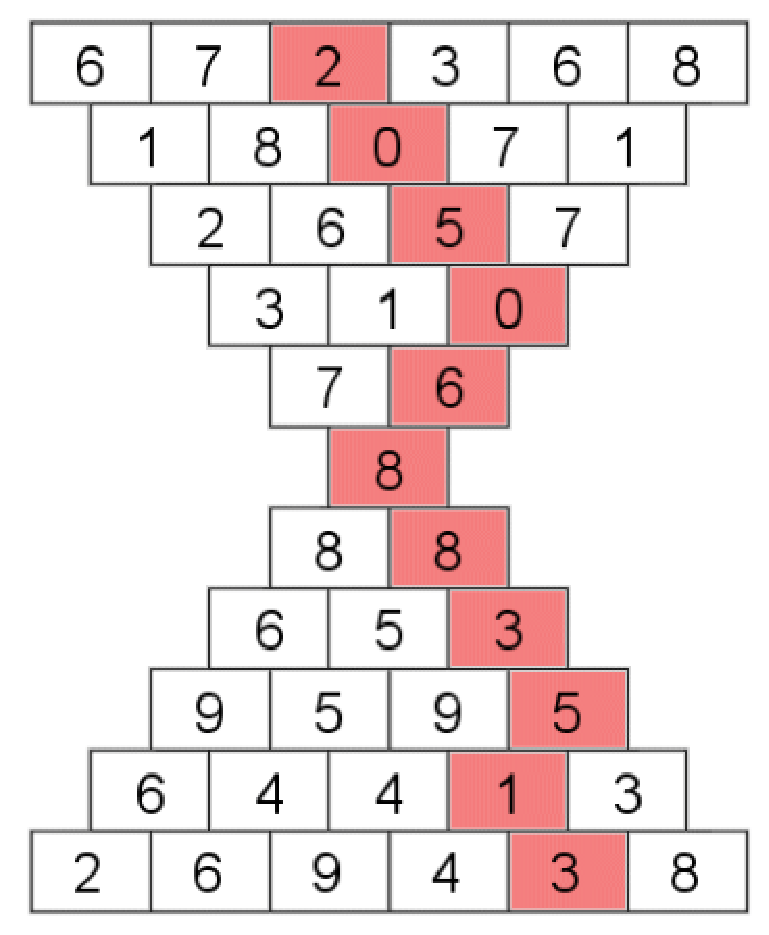
\includegraphics{Hourglass.pdf}
		}
	\caption{Example of a path in an hourglass}
	\end{figure}

	Describe an algorithm to find the path of maximum value through the hourglass. We shall use $n$ to denote the number of elements in the first and last row. An algorithm with worst-case running time in $\Theta(n^2)$ exists and your algorithm should have similar running time.

	Derive the runtime complexity of the algorithm and prove its correctness. \\

{\bf Solution.} Suppose that we started our path at row $i$ column $j$ (assuming the rows are numbered starting from the top and that the columns are numbered starting from the left). We will number the top-most row as row $-n+1$ where $n$ is the number of elements in that row. The row numbers increase until row $n-1$. Row $i$ has $|i|+1$ elements. We will use $H(i,j)$ to represent the value of cell $(i,j)$. Let $v(i,j)$ denote the maximum value that can be obtained if a path starts at cell $(i,j)$.

	The dynamic programming equation can be stated as follows:
	\[
		v(i,j) = \left \{ \begin{array}{ll}
								\max \{ v(i+1,j-1)+H(i,j), v(i+1,j)+H(i,j) \} & i < n, 1 \le j \le |i|+1 \\
								0 & i \ge n \\
								0 & j < 1 \\
								0 & j > |i|+1
							\end{array}
					\right.
	\]
	
	What we seek is $ \max_{1 \le j \le n} \{ v(-n+1,j) \}$.
	
	Using memoization, this problem can be solved in $O(n^{2})$ time.

\item Consider $n$ non-preemptable jobs $J_1, \dotsc, J_n$ that are all available (and ready to run) at time $0$. Job $J_i$ requires worst-case execution time $e_i \in \N$ and worst case (peak) memory requirement $M_i \in \N$ (in MB). Once assigned to processors, jobs cannot migrate to other processors. Moreover, the order of the jobs is fixed by the job dispatching system and so cannot be rearranged: In any allocation of processors to jobs, the jobs must appear in the same order as they are given in the input. Assume that the jobs are ordered according to their indices such that $J_{1}$ is the first job to be assigned, and if $i<j$ and $J_{i}$ is assigned processor $k$, then job $J_{j}$ must either execute on processor $k$ and start after $J_{i}$, or execute on the $(k+1)$st processor. The processors onto which the jobs are to partitioned are identical and 
each has maximum available time $L \in \N$; that is, the sum of execution times of the jobs assigned to any processor cannot exceed $L$. You may assume that $e_{i} \leq L$ for every $i \in \{1,\dotsc, n\}$.

Given an allocation of processors to the input jobs, the peak memory demanded by processor $\pi_{j}$ under the given allocation is defined as $\max\{M_i: J_{i} \text{ is assigned to processor } \pi_{j}\}$. Our goal is to assign the jobs to as many processors as needed, respecting the given processor available time and the no rearrangement constraint, so that the overall peak memory usage is minimized; that is, the sum of the peak memory used on all processors is kept at a minimum. Develop an algorithm to solve this problem optimally and prove its correctness. Derive the asymptotic running time of your algorithm in terms of $n, e_i, M_i$, and $L$ (or any subset thereof).  

\textbf{Solution.} We will do this with dynamic programming. Think about the way in which the jobs are placed on the processor. We can iteratively place the jobs on the processor where, at each step, we can make a decision to either place the job on the current processor, or to open a new processor. Sometimes, of course, we will have no choice: The processor may not be able to fit the job, and we would then be forced to open a new processor.
We will solve this problem first by going backwards. We will loop from $n$ down to 1 and determine the cheapest way (in terms of memory) of placing jobs $i$ through $n$ if we start a new processor with job $i$. We store the best costs in an array $\textsf{cost}$, where $\textsf{cost}[i]$ is the best possible memory cost of placing jobs $i$ through $n$. The recursion is the following:
\begin{align*}
  \textsf{cost}[i] = \min_{1 \leqslant k \leqslant m}\bigl \{ \textsf{cost}[i+k] + \max\{M_{i}, \dotsc, M_{i+k-1}\} \bigr\},
\end{align*}
where $m$ is the maximum integer such that $\sum_{j=i}^{m}e_{j} \leqslant L$. The base case is $\textsf{cost}[n]=M_{n}$. This recurrence can be converted to an iterative algorithm that runs in time $O(n^{2})$, which is \emph{strongly} polynomial.

% \item (Applying graph algorithms: 3 points.)

%   \begin{enumerate}    
    
%   \item (1 point) Find the shortest path between $s$ and $t$ in the following graph.
    
%     \begin{figure}[h]
%       \centering
%       \scalebox{0.7}{
%         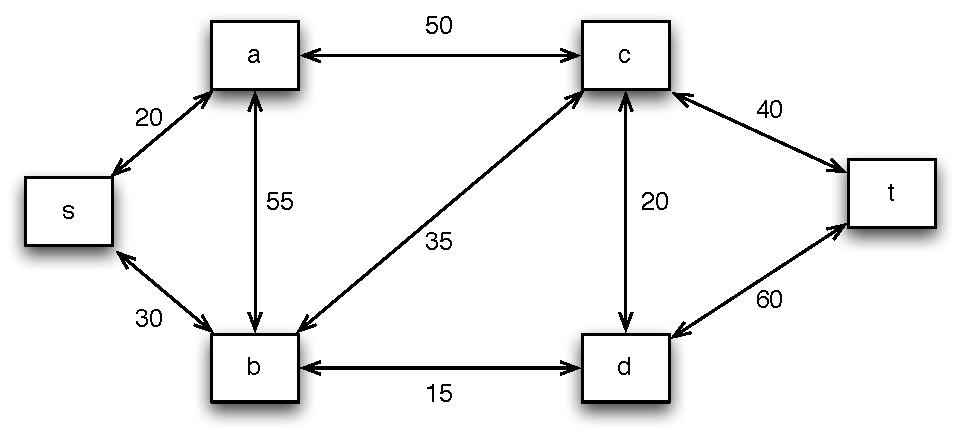
\includegraphics{Dijkstra.pdf}
%       }
%     \end{figure}

% \textbf{Solution.} 

% \begin{figure}[h]
%       \centering
%       \scalebox{0.7}{
%         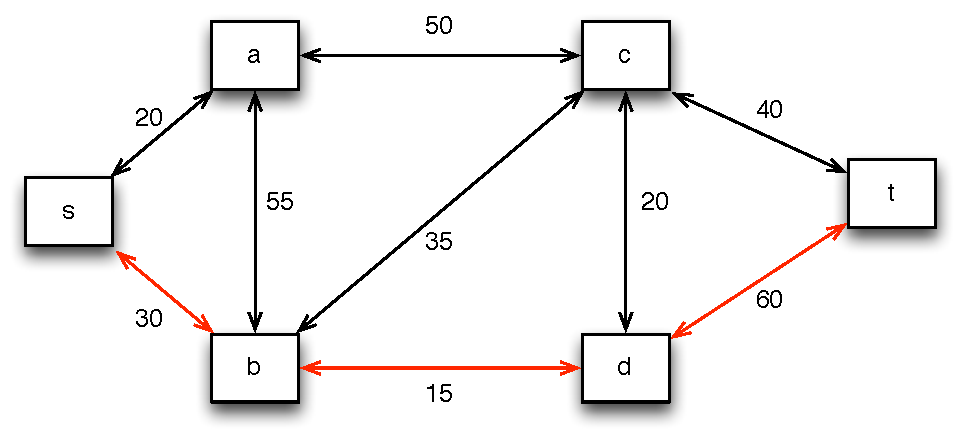
\includegraphics{Dijkstra-s.pdf}
%       }
%     \end{figure}

  

% \item (Directed acyclic graphs). A directed graph which has no directed cycles is called a directed acyclic graph (DAG). Note that the underlying undirected graph may have cycles.
%   \begin{enumerate}
%   \item Show that in any DAG, there is a vertex whose in-degree equals $0$, i.e., it is not the head for any edge. Such a vertex is called a \emph{source}.  
% \item Show that in any DAG, there is a vertex whose out-degree equals 0, i.e., it is not the tail for any edge. Such a vertex is called a \emph{sink}.

% \item Show that in any DAG, one can order the vertices so as to respect edge directions: i.e., show there exists a one-to-one and onto mapping $f : V (G) \to \{1, \dotsc, n\}$ such that for every directed edge $(u, v)$, $f (u) \leq f(v)$. So every edge points from a lower numbered vertex to a higher numbered vertex. This kind of an ordering is called a \emph{topological sort} of the vertices of a DAG.
% \item We say that a partition of the vertices $V = L_{0} \cup \dotsb \cup L_{k-1}$, where $L_{i} \cap L_{j} = \emptyset$ for all $i \neq j$, is a \emph{stratification} with $k$ levels, if every directed edge $e$ is between vertices in different levels, and the edge points from a lower indexed level to a higher indexed level. Notice that the topological sorting from the previous part is a stratification with $|V |$ levels. Let $G_{0}$ be a DAG and let $L_{0}$ be the set of sources in $G_{0}$. Consider the following graphs. For each $i = 1, 2, \dotsc,$ define $G_{i} = G_{i-1} \setminus L_{i-1}$ and $L_{i}$ is the set of sources in $G_{i}$. Notice that for some natural number $k^{*}$, for every $i \geq k^{*}$, $G_{i}$ is just the empty graph, i.e., empty set of vertices and empty set of edges. Show that $V = L_{0} \cup L_{1} \cup \dotsb L_{k^{*}-1}$ is a stratification.
% \item (\textbf{Bonus}) Show that $k^{*}$ in the previous part is the smallest $k \in \N$ such that there exists a stratification with $k$ levels.  
% \end{enumerate}


\end{enumerate}



%%%%%%%%%%%%%%%%%%%%%%%%%%%%%%%%%%%%%%%%%%%%%%%%%%%%%%%%%%%%%%%%%%%%%%%%%
%% the bibliography starts here.

%\newpage
%\bibliographystyle{acm}
%\setlength{\baselineskip}{0.8\baselineskip}
%\bibliography{../../Bibliography/CompleteBibliography}

%%%%%%%%%%%%%%%%%%%%%%%%%%%%%%%%%%%%%%%%%%%%%%%%%%%%%%%%%%%%%%%%%%%%%%%%%
%% other closing material

% \appendix
% \input{appendix.tex}

\end{document}
%%% Local Variables:
%%% mode: latex
%%% TeX-master: t
%%% End:
